Dans ce chapitre nous continuons nos travaux sur deux programmes malveillants particuliers, \duqu\ et \stux, dont nous avons montré qu'ils partageaient du code au chapitre précédent.
Notre objectif est de pouvoir détecter une attaque par \duqu\ connaissant \stux.
% cela nécessite un accès au code déchiffré et injecté par \duqu.

Nous cherchons donc à détecter \duqu\ avant qu'il ne puisse infecter une machine ciblée.
Nous avons pour cela étudié un composant spécifique de \duqu, son pilote (\emph{driver}) qui permet de charger discrètement le code malveillant en mémoire.
Notre contribution consiste en la rétroingénierie de ce composant, en la reconstitution de son code source et en une analyse de son fonctionnement.
Nous avons ensuite détourné le pilote pour en faire une version défensive capable de détecter d'éventuelles attaques similaires.
En particulier nous montrons comment le pilote de \duqu\ modifié permet de détecter et d'empêcher une attaque par \duqu.
Ces travaux ont fait l'objet d'une publication à SSTIC \cite{sstic13} ainsi qu'à  Malware \cite{mal13}.

\section{Détection d'une infection par Duqu}
\subsection{Déroulement d'une infection}
L'infection détectée par Crysys utilise un document Microsoft Word piégé, incluant \duqu.
Dans un premier temps il exploite une faille jusque là inconnue (\emph{0-day} sur les polices d'écriture TrueType \cite{CVETrueType}) du noyau Windows afin d'installer trois composants sur le système :
\begin{itemize}
 \item Un pilote : \driver
 \item Une DLL chiffrée : \netpDLL
 \item Un fichier de configuration chiffré : \netpCONF
\end{itemize}

Au redémarrage de la machine, le pilote surveille le chargement des processus par le système d'exploitation et injecte la DLL principale de \duqu, une fois déchiffrée, dans un processus spécifié par le fichier de configuration, typiquement \services.
Enfin le pilote modifie \services\ afin qu'il exécute la charge finale, qui est inclue dans la DLL.

Une fois installé sur une première cible, \duqu\ reçoit des ordres d'attaques et de propagation d'un serveur C\&C.
Chaque machine infectée peut être configurée pour se connecter à l'attaquant, pas directement mais par la machine qui l'a infectée, créant une sorte de tunnel de routage pour des machines non accessibles directement depuis l'extérieur. Une illustration de ce mécanisme est donnée en figure \ref{fig:propagationDuqu}.

\begin{figure}[h]
\begin{center}
 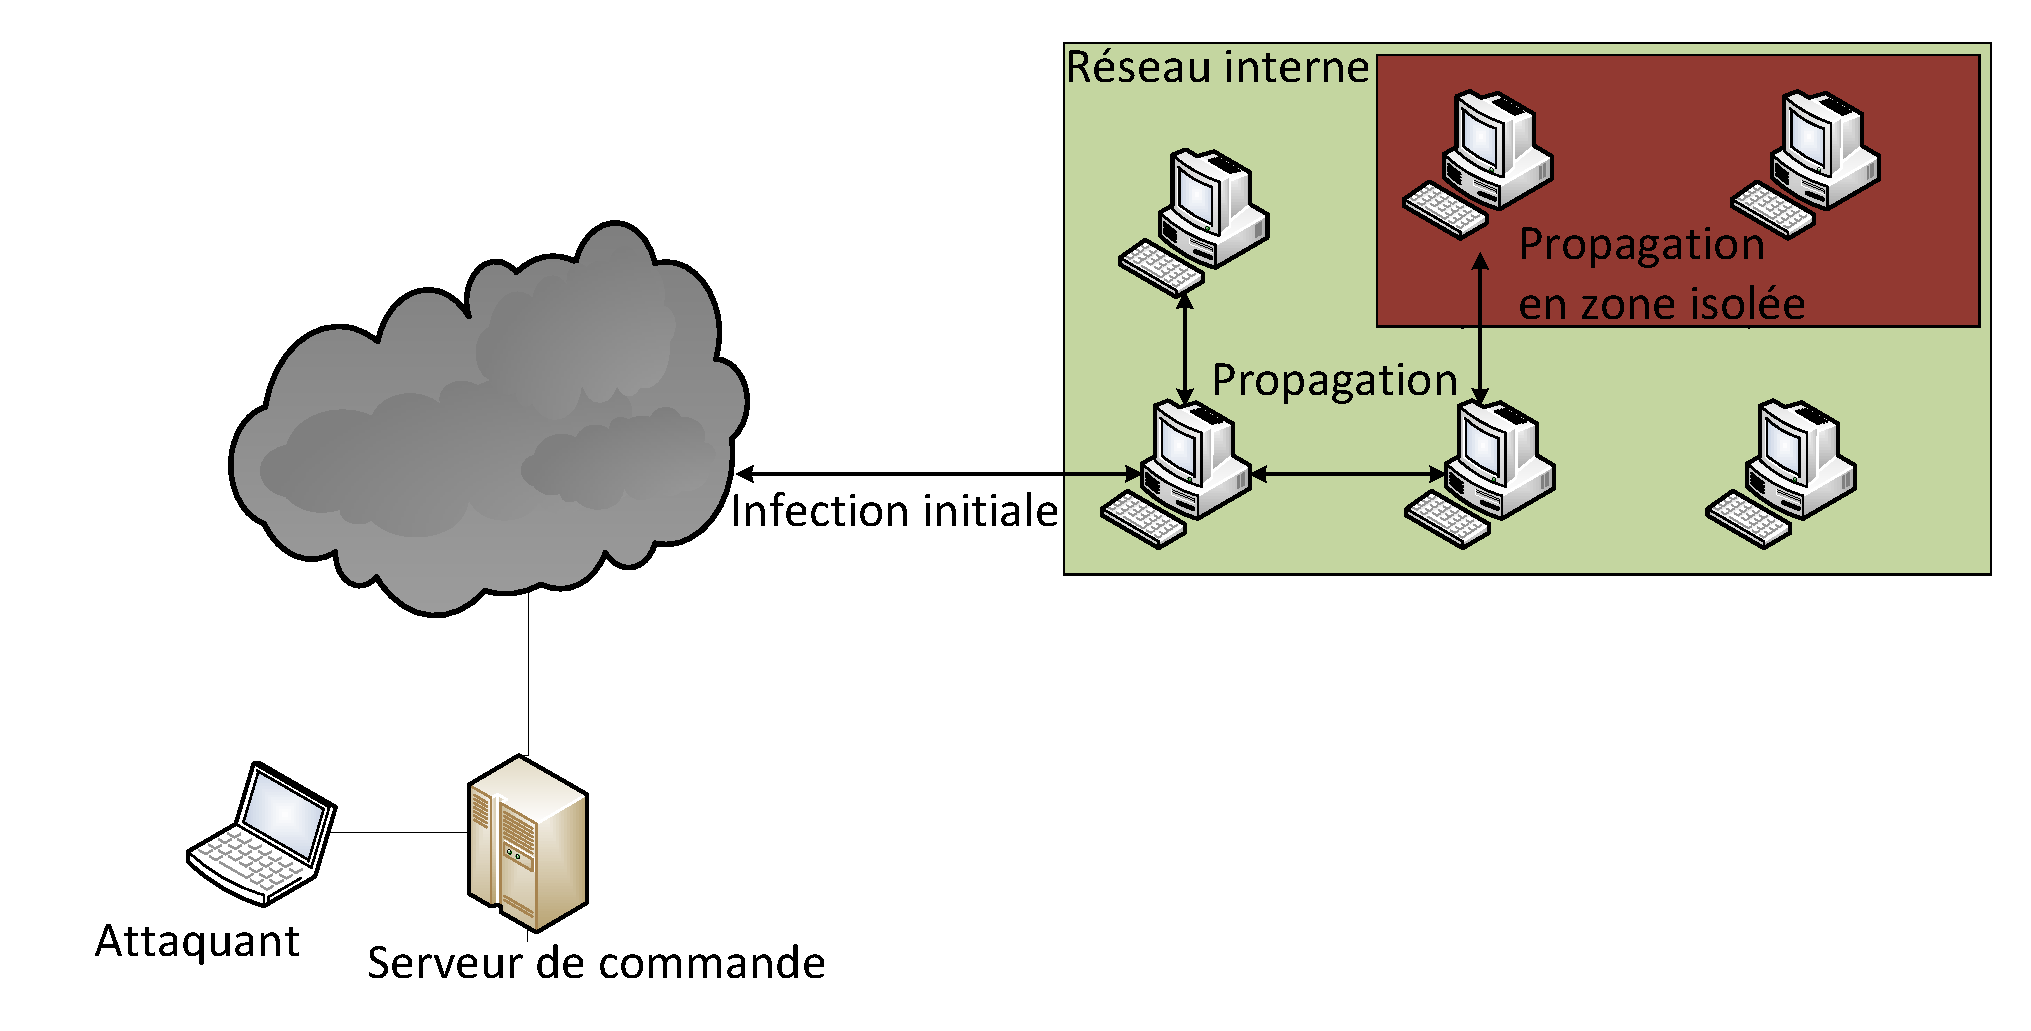
\includegraphics[width=0.8\textwidth]{supports/duqu/propagationDuqu.pdf}
 % graph11.eps: 0x0 pixel, 300dpi, 0.00x0.00 cm, bb=0 0 384 336
\end{center}
\caption{Schéma de propagation en profondeur de Duqu}
\label{fig:propagationDuqu}
\end{figure}

\paragraph{Difficulté de la détection.}
L'obstacle principal à la détection est que seul le pilote est présent déchiffré sur le disque.
La DLL est chiffrée et empaquetée avec UPX, elle n'apparaît déchiffrée qu'en mémoire, lorsqu'elle est injectée dans \services.

\paragraph{Angle d'attaque pour une détection.}
L'attaque peut être détectée au moment du déchiffrement de la DLL principale et de son injection.
Elle doit prendre place après le déchiffrement mais avant que la charge finale ne soit exécutée.
Nous aurons pour cela besoin de suivre les processus lancés et de pouvoir analyser les DLL qu'ils exécutent.
Étant donné que le pilote de \duqu\ réalise cette opération, nous avons choisi de le modifier de telle sorte qu'il puisse s'interfacer avec le détecteur par analyse morphologique.
Pour mettre ce plan en \oe uvre, nous avons
\begin{itemize}
 \item reconstitué, par rétroingénierie, le code source du pilote de \duqu\ à partir de son binaire.
 \item modifié son code pour qu'il surveille le chargement des processus sans provoquer d'injection.
%  \item Interfacé le nouveau pilote avec notre outil de détection.
\end{itemize}

\subsection{Reconstruction du code du pilote}
Nous savions donc que les DLL principales de \duqu\ et \stux\ partagent du code.
Le pilote de \stux\ a été décompilé par Amr Thabet \cite{ThabetDriver}.
Nous avons voulu suivre la même route et désassembler le pilote de \duqu\ afin de le documenter.
Nous avions à notre disposition la souche du pilote découverte en octobre 2011 en Europe : \driver.

Nous avons donc travaillé sur la rétroingénierie de cette version spécifique du pilote afin d’en documenter les fonctionnalités. 
Notre objectif est d’obtenir un code compréhensible, que l'on peut compiler, et dont la version compilée soit au plus proche du binaire d'origine.

\subsubsection{Décompilation avec IDA}
Nous avons utilisé le module de décompilation "Hex-Rays Decompiler", intégré à IDA sous la forme d’un greffon \cite{IDADecompiler}.
Il permet de générer un pseudo-code C à partir du fichier binaire en cours d’analyse.
Il produit non seulement du code source mais facilite également sa réécriture directement à l’intérieur de l’interface graphique du greffon. 
Malheureusement le code en sortie n’est, dans notre cas, pas exploitable directement. 
D’une part le code n’est pas compilable parce que des types de variables n’ont pas été correctement reconnus et certaines conventions d’appel ne sont pas standard (non reconnues par le décompilateur). 
De plus le code généré est difficilement lisible, en partie parce que certaines structures n’ont pas été identifiées.
Nous détaillerons dans les paragraphes suivants ces difficultés et des moyens de résolution.

Nous avons procédé de manière incrémentale afin de reconstruire le code petit à petit en vérifiant à chaque étape que le code compile et qu'une fois compilé il est équivalent à celui du binaire \driver\ original. 
Cela a consisté à :
\begin{itemize}
 \item commenter tout le pseudo-code sauf la fonction du point d'entrée du pilote (\emph{DriverEntry}) et les variables globales s'y rapportant,
 \item régler chaque erreur une par une,
 \item comparer le code compilé au binaire original, modifier le code pour s'en rapprocher,
 \item ajouter du code auparavant commenté et revenir à l'étape de correction d'erreurs.
\end{itemize}

\subsubsection{Identification des structures et des types}
La figure \ref{fig:ParsePEInitial} montre les premières lignes du code C reconstruit par le décompilateur pour une des fonctions du pilote.
Beaucoup d'informations manquent. Par exemple la plupart des types sont décrits comme des entiers (ou des pointeurs) : il n'est pas possible de savoir quel type de données cette fonction manipule.
Nous allons détailler sur cet exemple quelques techniques permettant de récupérer ces informations.

\begin{figure}[h]
\begin{center}
\begin{lstlisting}[language={C}]
signed int __cdecl sub_12F36(int a1, int a2, int a3)
{
  int v4; // eax@3
  unsigned __int16 v5; // cx@4
  int v6; // ecx@7

  v4 = a2 + *(_DWORD *)(a2 + 60);
  if (*(_DWORD *)v4 ^ 0xF750F284 != 0xF750B7D4)
    return 1;
\end{lstlisting}
\end{center}
\caption{Premières lignes de la fonction ParsePE décompilée par IDA\label{fig:ParsePEInitial}}
\end{figure}

Certaines constantes peuvent nous aider : par exemple \texttt{0xF750F284 XOR 0xF750B7D4 = 0x00004550} , qui représente la chaîne de caractères 'PE$\backslash$0$\backslash$0' en ASCII. Le texte était obscurci à l'aide d'une opération de ou exclusif (\emph{XOR}).

Nous soupçonnons alors que cette fonction est utilisée pour le traitement de fichiers binaires au format PE.
La documentation officielle de Microsoft Visual C++ détaille la structure PIMAGE\_NT\_HEADERS dont le premier champ, \emph{Signature}, vaut \PEzz\ pour les binaires Windows.
Ainsi la variable \texttt{v4}, qui est comparée à \PEzz, est probablement du type PIMAGE\_NT\_HEADERS.
Nous forçons ce type pour cette variable au sein d'IDA, à la place du type \texttt{int} et IDA trouve automatiquement le nom des champs de ce type de variable à partir de leur décalage (\emph{offset}) en mémoire.
Lorsque les structures sont spécifiques au binaire analysé, il est possible de les définir manuellement dans le décompilateur.
Nous avons retrouvé les types des autres variables de manière similaire.

La figure \ref{fig:ParsePEFinal} donne les premières lignes de la fonction retouchée.
Elle est lisible par un développeur C : on peut voir que la fonction vérifie si un fichier est binaire PE.
Le reste de la fonction parcourt le binaire PE passé en entrée et remplit une structure spécifique avec quelques informations (son point d'entrée, ses sections, etc.).
De plus le code compilé de cette fonction est très similaire au binaire d'origine.


\begin{figure}[h]
\begin{center}
\begin{lstlisting}[language={C}]
NTSTATUS __cdecl ParsePE(__out PEDataPtr pPEData, 
    __in PIMAGE_DOS_HEADER BaseAddress, __in int flag){
PVOID infosPE;
PIMAGE_DOS_HEADER pDosHeader;
PIMAGE_NT_HEADERS pNtHeader;

pNtHeader = (DWORD)infosPE + infosPE->e_lfanew;
if ((pNtHeader->Signature ^ 0xF750F284) 
      != (IMAGE_NT_SIGNATURE ^ 0xF750F284)) 
    return STATUS_WAIT_1; 
\end{lstlisting}
\end{center}
\caption{Premières lignes de la fonction ParsePE reconstruite\label{fig:ParsePEFinal}}
\end{figure}

\subsubsection{Conventions d'appel}

Pour chaque routine IDA cherche à déterminer la convention d'appel utilisée à partir des registres qui sont lus avant d'être écrits (paramètres) et ceux écrits sans être lus après (valeur de retour). Si ces registres correspondent à un appel classique, IDA l'annote dans le code C pour que le compilateur respecte la convention. Les conventions d'appel de Microsoft Visual C++ sont données Figure \ref{fig:callingconvention}, l'appel par défaut étant \emph{thiscall}. Dans le cas où il ne détermine pas la convention, il annote les registres d'entrée et de sortie en notant qu'il s'agit d'un appel non conventionnel (\emph{usercall}) et met la définition de la fonction en commentaire (ici les arguments sont passés dans les registres \texttt{edi} et \texttt{esi}) :
\begin{small}
\begin{lstlisting}[language={C}, escapechar=!]
!//! int __usercall SearchForCode<eax>(int *a1<edi>, int a2<esi>);
\end{lstlisting}
\end{small}

Une convention d'appel non standard est détectée dans le cas où une partie de la fonction a été écrite directement en assembleur ou à la suite d'une optimisation faite par le compilateur. On doit alors réécrire, en partie en assembleur, la fonction sans passer par le décompilateur ou choisir une convention d'appel soi-même.

\begin{figure}[h]
\begin{center}
\begin{tabular}{|l|c|c|c|c|}
\hline 
Convention & Arguments & \emph{this} (C++) & Retour & Nettoie la pile\\
\hline
C (\_\_cdelcl) & pile & (argument) & eax & appelant\\
Standard (\_\_stdcall) & pile & (argument) & eax & appelé\\
Thiscall (\_\_thiscall) & pile & ecx & eax & appelé\\
Fastcall (\_\_fastcall) & ecx, edx, pile & (argument) & eax & appelé\\
\hline
\end{tabular}
\end{center}
\caption{Conventions d'appel dans leur version Visual C++}
\label{fig:callingconvention}
\end{figure}

Nous avons réalisé ce type d'analyse sur l'ensemble du pilote afin d'en reconstruire une version compréhensible et cohérente du code source du pilote.

\section{Analyse fonctionnelle du pilote de Duqu à partir du code source}
Une fois le code du pilote reconstitué, nous l'avons donc analysé.
Il y a deux phases principales, la première consiste en la mise en place du pilote : il demande au système à être notifié en cas de chargement de binaires et initialise ses mécanismes de furtivité.
La seconde phase est lancée lorsqu'une notification est signalée au chargement d'un des binaires ciblés : le pilote infecte alors le binaire en y injectant la DLL du \duqu\ puis celle-ci active la charge finale.

\subsection{Initialisation du pilote lors du démarrage du système}
Sous Windows l'ordre de démarrage des pilotes est déterminé par leur clé de registre \texttt{Group}.
Le pilote \driver\ de \duqu, appartenant au groupe ``network'', est activé avant même que la couche d'abstraction matérielle (\emph{HAL}) ne soit chargée en mémoire.

Le pilote, une fois démarré, commence par allouer un emplacement mémoire de 512 octets destiné à contenir un tableau de pointeurs de fonctions partagées entre les différentes routines de rappel (\emph{callback}) qui seront définies par la suite.
Il passe ensuite au déchiffrement de quelques paramètres internes, révélant le nom et l'emplacement de la clé de registre utilisée pour la configuration de l'injection.

Si le déchiffrement s'est correctement déroulé, vient alors la vérification du mode d'exécution : soit le système s'avère être en mode sans échec ou en mode débogage, dans ce cas le pilote termine prématurément son exécution ; soit il est en mode normal et il crée alors un \emph{device}, \texttt{\{624409B3-4CEF-41c0-8B81-7634279A41E5\}}, et définit la liste des commandes de contrôle qu'il sera amené à traiter.

Cette étape réalisée, le pilote enregistre deux fonctions de rappel auprès du gestionnaire d'événements interne du noyau.
La première est requise par le système : elle est utilisée pour créer un point d'accès ($\backslash$\texttt{Device}$\backslash$\texttt{Gpd0}) et un lien ($\backslash$\texttt{DosDevices}$\backslash$\texttt{GpdDev}) vers le pilote, ainsi que pour définir une pile mémoire pour le \emph{device}.
La seconde fonction sera appelée lorsque le pilote sera initialisé ou ré-initialisé. 


Cette seconde fonction attend que le noyau Windows soit complètement chargé en vérifiant si la DLL \texttt{hal.dll} est chargée en mémoire. Lorsque le système est prêt, un point d'accès, $\backslash$\texttt{Device}$\backslash$\texttt{Gpd1}, est créé et lié à une routine de traitement des requêtes. 
À ce stade le pilote est prêt à réaliser l'injection.

\subsubsection{Techniques de furtivité}
Le pilote agit désormais furtivement (on parle de \emph{rootkit}) et évite d'utiliser directement des appels systèmes connus pour être sensibles, utilisés par des logiciels malveillants, et probablement surveillés par un éventuel antivirus.
La fonction \ZwA\ peut être utilisée pour allouer de la mémoire au sein d'un processus au choix, pour y injecter du code arbitraire par exemple.
De plus, afin de détourner le point d'entrée d'un binaire (\emph{hook}), \duqu\ veut également utiliser la fonction \ZwP\ que Microsoft a délibérément omise de la liste des fonctions accessibles en dehors du noyau. Cette fonction permet de modifier les permissions d'une page mémoire et peut être utilisée pour rendre une partie de code accessible en écriture ou rendre une section de données exécutable.

Ces deux fonctions sont implémentées dans le noyau Windows, dans les fichiers \path{Ntoskrnl.exe} ou \path{ntkrnlpa.exe}, selon les versions. 
Le pilote inspecte chaque module, DLL et exécutables, chargés par le système lors du démarrage à la recherche d'un de ces deux fichiers.

Une fois le fichier cible trouvé, le pilote utilise la fonction \emph{ParsePE} pour l'examiner et y retrouver l'adresse de \ZwP.
Pour cela il dispose d'un motif à reconnaître.
Il est à la recherche d'un appel vers \ZwA, dont l'adresse est connue parce qu'elle est présente dans la table d'exports du noyau, suivi par l'instruction \texttt{push 0x104} et par une instruction \texttt{call}.
Si ce motif, représenté en figure \ref{fig:CallZwProtect}, est retrouvé alors l'adresse cible de ce \texttt{call} est considérée comme étant \ZwP.
À partir de cet instant, le pilote connaît les adresses mémoires de ces deux fonctions.

\begin{figure}[h]
\begin{center}
\scriptsize
\begin{lstlisting}[language={[x86masm]Assembler}, escapechar=~]
(01) PAGE:004ED1AD                  loc_4ED1AD: [...]                      
(02) PAGE:004ED1BC 50               push    eax             ; BaseAddress
(03) PAGE:004ED1BD 57               push    edi             ; ProcessHandle
(04) PAGE:004ED1BE E8 19 8C F1 FF   ~\textcolor{red}{\texttt{call    DS:ZwAllocateVirtualMemory}}~
(05) PAGE:004ED1C3 3B C3            cmp     eax, ebx
(06) PAGE:004ED1C5 8B 4D FC         mov     ecx, [ebp+BaseAddress]
(07) PAGE:004ED1C8 89 4E 0C         mov     [esi+0Ch], ecx
(08) PAGE:004ED1CB 7C 2E            jl      short loc_4ED1FB
(09) PAGE:004ED1CD 38 5D 0B         cmp     byte ptr [ebp+ProcessHandle+3], bl
(10) PAGE:004ED1D0 74 27            jz      short loc_4ED1F9
(11) PAGE:004ED1D2 8B 45 D0         mov     eax, [ebp+var_30]
(12) PAGE:004ED1D5 89 45 F8         mov     [ebp+ProtectSize], eax
(13) PAGE:004ED1D8 8D 45 F4         lea     eax, [ebp+OldProtect]
(14) PAGE:004ED1DB 50               push    eax             ; OldProtect
(15) PAGE:004ED1DC 68 04 01 00 00   ~\textcolor{red}{\texttt{push    104h}}~
(16) PAGE:004ED1E1 8D 45 F8         lea     eax, [ebp+ProtectSize]
(17) PAGE:004ED1E4 50               push    eax             ; ProtectSize
(18) PAGE:004ED1E5 8D 45 FC         lea     eax, [ebp+BaseAddress]
(19) PAGE:004ED1E8 50               push    eax             ; BaseAddress
(20) PAGE:004ED1E9 57               push    edi             ; ProcessHandle
(21) PAGE:004ED1EA E8 93 96 F1 FF   ~\textcolor{red}{\texttt{call    loc\_406882}}~ ; ZwProtectVirtualMemory
(22) PAGE:004ED1EF 3B C3            cmp     eax, ebx
\end{lstlisting}
\end{center}
% \end{framed}
\caption{Fonction faisant appel à \ZwP\label{fig:CallZwProtect}}
\end{figure}

\paragraph{Vérification d'intégrité.}
Le pilote cherche à détecter si les fonctions \ZwA\ et \ZwP\ ont été la cible d'un détournement défensif par un antivirus cherchant à les surveiller.
Il vérifie dans un premier temps que les deux fonctions sont présentes dans l'espace mémoire du noyau et non en espace utilisateur.
Dans un second temps il leur applique un masque d'intégrité vérifiant la valeur d'une partie des 20 premières adresses mémoires sur lesquelles les deux fonctions sont codées. Le masque est le même pour les deux fonctions et est donné en figure \ref{fig:masque_integrite}.
Si les fonctions passent le test, leurs adresses sont considérées valides et sont conservées pour une future utilisation discrète.


\begin{figure}[h]
\begin{center}
% Masque d'intégrité :\\
\begin{tabular}{|c|c|c|c|c|c|c|c|c|c|}
\hline
b8\cgris & ~~ & ~~ & ~~ & ~~ & 8d\cgris & 54\cgris & 24\cgris & 04\cgris & 9c\cgris \\
\hline
6a\cgris & 08\cgris & e8\cgris & ~~ & ~~ & ~~ & ~~ & c2\cgris & 14\cgris & ~~\\
\hline
\end{tabular}
\end{center}

\begin{center}
\ZwA:\\
\begin{tabular}{|l|c|c|c|c|c|l|}
\hline
\adr{405ddc} & b8\cgris & 11 & 00 & 00 & 00 & mov eax, 0x11 \\
\hline
\adr{405de1} & 8d\cgris & 54\cgris & 24\cgris & 04\cgris & ~~ & lea edx, [esp+ProcessHandle] \\
\hline
\adr{405de5} & 9c\cgris & ~~ & ~~ & ~~ & ~~ & pushf \\
\hline
\adr{405de6} & 6a\cgris & 08\cgris & ~~ & ~~ & ~~ & push 8 \\
\hline
\adr{405de8} & e8\cgris & b9 & 20 & 00 & 00 & call +0x20be (sub\_407ea6) \\
\hline
\adr{405ded} & c2\cgris & 14\cgris & 00 & ~~ & ~~ & ret 0x14 \\
\hline
\end{tabular}
~\\~\\
\ZwP:\\
\begin{tabular}{|l|c|c|c|c|c|l|}
\hline
\adr{406882} & b8\cgris & 89 & 00 & 00 & 00 & mov eax, 0x89 \\
\hline
\adr{406887} & 8d\cgris & 54\cgris & 24\cgris & 04\cgris & ~~ & lea edx, [esp+ProcessHandle] \\
\hline
\adr{40688b} & 9c\cgris & ~~ & ~~ & ~~ & ~~ & pushf \\
\hline
\adr{40688c} & 6a\cgris & 08\cgris & ~~ & ~~ & ~~ & push 8 \\
\hline
\adr{40688e} & e8\cgris & 13 & 16 & 00 & 00 & call +0x1618 (sub\_407ea6) \\
\hline
\adr{406893} & c2\cgris & 14\cgris & 00 & ~~ & ~~ & ret 0x14 \\
\hline
\end{tabular}
\end{center}

\caption{Masque d'intégrité appliqué à \ZwA\ et \ZwP. Les valeurs grisées sont celles qui sont vérifiées.}
\label{fig:masque_integrite}
\end{figure}

\FloatBarrier
\subsubsection{Initialisation de la mémoire partagée}
Une mémoire partagée est allouée et utilisée comme lien entre les routines de rappel du pilote et le noyau.
Elle contiendra, entre autres, les paramètres pour l'infection déchiffrés depuis les données d'une clé de registre et une table d'imports donnant accès à la DLL \texttt{kernel.dll} et aux fonctions du noyau.
Cette table d'imports sera utilisée à la fois par le code que \duqu\ va injecter dans \services\ et par la charge finale.

La phase d'initialisation prend fin en mettant en place une notification système dès qu'un module (DLL ou exécutable) est chargé en mémoire, via l'appel système \textbf{PsSetLoadImageNotifyRoutine}.

\FloatBarrier
\subsection{Injection de code}
\subsubsection{Traitement de la première notification}
\paragraph{Préparation à l'injection.}
Le pilote est notifié à chaque fois qu'un module (DLL ou exécutable) est chargé en mémoire.
À chaque fois le pilote tente de localiser l'emplacement mémoire du module.
Pour cela il utilise l'identifiant du processus que lui fournit le système d'exploitation lors de la notification.
Il lit l'adresse de base du fichier directement à partir des informations accessibles dans la structure PEB (\emph{Process Environment Block}) et la compare à celle passée en paramètre par le système.
Il vérifie que le fichier de configuration est bien déchiffré dans la mémoire partagée et lit le champ donnant la cible de l'injection.
Comme expliqué dans le document de Crysys \cite{CrysysDuquStuxnet}, la cible est \services\ donc nous nous focaliserons sur ce processus et l'injection dont il sera victime.

\paragraph{Injection de la charge finale.}
Le pilote de \duqu\ va maintenant injecter du code malveillant dans \services\ de telle manière que la charge finale soit exécutée par \services\ avant que son code légitime ne soit à son tour exécuté.

Une fois que \services\ est chargé, le pilote détermine son point d'entrée et alloue de la mémoire dans sa section \pdata\ à l'aide de la fonction \ZwA.
Deux fichiers PE dont les entêtes ont été altérés, à des fins de furtivité, sont injectés.
Ensuite certaines constantes ('\texttt{MZ}', '\texttt{IMAGE\_NT\_SIGNATURE}', '\texttt{IMAGE\_PE\_i386\_MACHINE}, et '\texttt{IMAGE\_PE32\_MAGIC}') du premier code injecté sont restaurées.
Certaines adresses sont recalculées : les adresses cibles de sauts qui étaient codées en dur doivent être recalculées.
Enfin le pilote modifie les permissions du point d'entrée de \services\ de \texttt{RX} (\texttt{PAGE\_EXECUTE\_READ}) à \texttt{RWX} (\texttt{PAGE\_EXECUTE\_WRITECOPY}) en utilisant la fonction \ZwP.

Le pilote \driver\ alloue alors de la mémoire dans le processus \services\ de la taille de la DLL déchiffrée \netpDLL\ augmentée de 57 octets.
Ensuite un gestionnaire d’événements (\emph{handler}) est ouvert sur le pilote et est sauvegardé dans la mémoire partagée afin de pouvoir être utilisé par le code injecté.

\subsubsection{Traitement de la seconde notification}
Le pilote n'est pas uniquement notifié quand le module principal (\services) est chargé mais également lorsque des DLL liées à ce module sont également chargées.
\idone{Les sigles ne prennent pas la marque du pluriel}
En particulier lorsque la DLL \texttt{kernel32.dll} est chargée, le pilote cherche les adresses de 10 de ses fonctions exportées qui seront utilisées par la charge finale.
Toujours dans une optique de furtivité la recherche consiste à comparer un haché cryptographique au nom de chacune des fonctions exportées par la DLL.
Cette étape se termine par une sauvegarde des 12 premiers octets présents au point d'entrée de \services\ et leur remplacement par un saut vers le premier code injecté et restauré.
Les premières instructions du point d'entrée sont changées en l'instruction \texttt{mov eax, @AdresseInjection} suivie de \texttt{call eax}.

Le processus \services\ a ainsi été altéré et est prêt à lancer la charge finale.

\subsubsection{Lancement de la charge finale}
Le système d'exploitation termine l'initialisation de \services\ et procède à son exécution en passant le contrôle au point d'entrée modifié, c'est à dire au premier code injecté par \duqu.

Sa première tâche consiste à déterminer sa propre adresse en mémoire afin de pouvoir recalculer les adresses de certaines cibles de saut.
Cette opération peut être effectuée à l'aide de deux instructions : un \texttt{call +5} vers l'instruction suivante suivi d'un \texttt{pop eax} a pour effet de placer l'adresse de retour (celle de \texttt{pop eax}) en haut de la pile, puis de la dépiler dans \eax\ qui contient alors cette même adresse.
Il modifie alors les adresses à partir du nouveau point d'entrée déterminé.

Il restaure ensuite les entêtes du second PE injecté afin de le rendre valide et remplit, dans une structure partagée, une table d'import à partir des 10 fonctions trouvées précédemment de \texttt{kernel32.dll}.
Il crée ensuite un gestionnaire d’événements sur la DLL \texttt{ntdll.dll} qui est enregistré dans une structure partagée.
Il transfert ensuite le contrôle au point d'entrée sur second code injecté.

Ce module additionnel ajoute les données de son propre entête (adresse du module, nombre de sections, adresse de la table d'exports) dans la mémoire partagée.
Enfin ces informations sont utilisées pour charger ce PE manuellement en mémoire : les espaces mémoires sont alloués, l'entête est copié, les sections et les DLL liées sont chargées en mémoire, une table d'imports est créée, les adresses sont recalculées à partir de son point d'entrée.
Puis la DLL principale de \duqu, \netpDLL, est chargée et liée à ce PE et son point d'entrée est appelé.
La figure \ref{fig:ServiceMem} donne l'état du processus \services\ et de la mémoire à cette étape de l'injection.


\begin{figure}[h]
\begin{center}
\scalebox{1}{
\begin{tikzpicture}[->,scale=1,>=stealth',thick]
\node[state, align=left, text width=6cm, minimum size=1cm] (EP){\small Point d'entrée altéré:\\\adr{01012475} \texttt{mov eax, 0x0a18bd}\\\adr{0101247a} \texttt{call eax}};
\node[state, below=-0.05cm of EP.south, anchor=north, text width=6cm, minimum size=1cm] (TEXTP){...};
\node [fit={($(EP.north west) + (0.0, 0.4)$) ($(TEXTP.south east) + (0.0, 0.0)$)}, draw, dash pattern=on \pgflinewidth off 2pt, label={[xshift=1.2cm,yshift=-0.55cm]north west:\small Code}](TEXT) {};

\node[state, below=1cm of TEXTP.south, anchor=north, text width=6cm, minimum size=0.7cm] (PE1){PE injecté avec entêtes restaurés};
\node[state, below=0.1cm of PE1.south, anchor=north, text width=6cm, minimum size=0.7cm] (PE2){PE injecté avec entêtes restaurés};
\node [fit={($(PE1.north west) + (0.0, 0.4)$) ($(PE2.south east) + (0.0, 0.0)$)}, draw, dash pattern=on \pgflinewidth off 2pt, label={[xshift=1.7cm,yshift=-0.55cm]north west:\small Données}](DATA) {};

\node[state, below=1cm of PE2.south, anchor=north, text width=6cm, minimum size=0.7cm] (DLL){DLL déchiffrée};
% \node[state, below=0.1cm of PE1.south, anchor=north, text width=6cm, minimum size=0.7cm] (PE2){PE injecté avec entêtes restaurés};
\node [fit={($(DLL.north west) + (0.0, 0.4)$) ($(DLL.south east) + (0.0, 0.0)$)}, draw, dash pattern=on \pgflinewidth off 2pt, label={[xshift=0.9cm,yshift=-0.55cm]north west:\small Tas}](TAS) {};
\node [fit={($(TEXT.north west) + (0.0, 0.0)$) ($(TAS.south east) + (0.0, 0.0)$)}, draw, label=\services](SERVICES) {};

\node[state, right=1cm of SERVICES.east, anchor=west, text width=6cm, minimum size=0.7cm] (DUQUPE){PE};
\node[state, below=0.1cm of DUQUPE.south, anchor=north, text width=6cm, minimum size=0.7cm] (DUQUDLL){DLL};
\node [fit={($(DUQUPE.north west) + (0.0, 0.0)$) ($(DUQUDLL.south east) + (0.0, 0.0)$)}, draw, label=Charge finale de \duqu](DUQU) {};

% \node[state, text width=2cm, minimum size=3cm] (TEXT){Code};
% \node[state, below = -3cm of TEXT.north, text width=2cm, minimum size=3cm, anchor=north] (DATA){Données};
% \draw ($(BIN.east) + (0.5, 0) $) -- node[below]{\large Enpaquetage} ($(BIN.east) + (3cm, 0) $);
% \node [fit={($(UNPACK.north west) + (-0.1, 0.1)$) ($(BINO.south east) + (0.1, -0.1)$)}, draw, label=Binaire empaqueté] {};
\end{tikzpicture}
}
\end{center}
\caption{Mémoire de \services\ et de \duqu\ une fois que l'injection est complète}
\label{fig:ServiceMem}
\end{figure}

La charge finale contenue dans la DLL est maintenant en place et exécutée.
Une fois qu'elle a fini, elle envoie une requête au pilote via le point d'accès créé précédemment, \texttt{\{624409B3-4CEF-41c0-8B81-7634279A41E5\}}, afin qu'il restaure les 12 premiers octets du point d'entrée de \services.
Une seconde requête est envoyée pour restaurer les droits d'accès d'origine du point d'entrée de \services.

L'attaque ayant été réalisée, le contrôle est maintenant passé à \services, qui a été restauré et s'exécute cette fois normalement.

\section{Réalisation d'une version défensive}
Nous avons précédemment décrit comment la DLL de \duqu\ est injectée dans \services.
Certaines des techniques décrites, telle la mise en place de notifications au lancement de chaque module, peuvent être utilisées à des fin défensives.

Schématiquement, le pilote modifié va calculer des signatures sur les binaires chargés en mémoire.
Lorsqu'un binaire est lancé, dans le cas où sa signature n'est pas reconnue, il sera considéré suspect et stoppé.
Nous détaillons les phases d'initialisation, de mémorisation puis de détection implémentées dans le pilote modifié.
Nous terminerons ce chapitre par une présentation détaillée d'une exécution du binaire modifié en situation d'attaque par \duqu.

\subsection{Phase d'initialisation}
La phase d'initialisation d'origine a été grandement allégée pour notre pilote modifié.
Nous avons gardé la création des points d'accès, enlevé la recherche de la fonction \ZwP, que nous n'utiliserons pas.
Nous avons conservé le système de notification des chargements de modules en mémoire et avons également demandé à recevoir une notification lorsque le système termine la création d'un processus (à l'aide de la fonction \emph{PsSetCreateProcessNotifyRoutine}).

\subsection{Phase de mémorisation}
Nous avons vu que le point d'entrée n'est pas altéré lors de la première notification.
Ainsi si une somme de contrôle est calculée pour le point d'entrée de chaque module, la modification du point d'entrée pourra être détectée lorsque la seconde notification sera déclenchée.
Nous avons intégralement repris la fonction de hachage implémentée dans \duqu\ qui était à l'origine utilisée pour obscurcir le nom des fonctions appelées.

Une première notification est reçue lorsque le processus est créé.
% Malheureusement Windows fournit uniquement l'identifiant du processus et son processus parent, mais pas d'informations sur l'emplacement en mémoire du processus.
Nous récupérons la structure PEB (\emph{Process Environment Block}) associée à ce processus et l'utilisons pour récupérer l'adresse mémoire du module chargé.

Afin de détecter \duqu\ nous nous focalisons uniquement sur le processus \services\ ciblé.
Si le nom du processus chargé est ``\services '', nous recherchons son point d'entrée, nous calculons une somme de contrôle sur ses huit premiers octets et l'enregistrons comme signature initiale.
Le pilote défensif est maintenant prêt à détecter l'injection effectuée par \duqu.

\subsection{Phase de détection}
Lorsqu'un module est chargé, le système passe le contrôle au pilote défensif qui vérifie le point d'entrée du module.
Si le module est une DLL, le point d'entrée recherché est celui de l'exécutable auquel la DLL est associée.
Nous avons donc ajouté une vérification de la somme de contrôle.

Cette somme de contrôle est comparée à celle calculée en premier lieu.
Si elles diffèrent, nous considérons qu'une injection a eu lieu sur \services\ entre les deux notifications et, puisque son point d'entrée a été altéré, le processus \services\ est considéré comme suspect.


\subsection{Démonstration}
Pour faciliter la mise au point du pilote de détection, nous l'avons installé, ainsi que celui de \duqu, sur une machine de test en suivant la démarche proposée par Sergei Shevchenko \cite{SShevchenko}.
Nous renommons la calculatrice Windows (\texttt{calc.exe}) en \services\ et observons comment deux pilotes réagissent à son lancement.

Pour cette démonstration, nous avons utilisé deux machines virtuelles sous Windows XP SP3 connectées par un lien série.
Une instance de WinDbg \cite{WinDbg}, débogueur fonctionnant sur le noyau Windows, tourne sur la première machine.
La seconde machine est lancée en mode ``débogage du noyau'' l'autorisant à dialoguer avec la première machine afin que celle-ci puisse déboguer les pilotes du noyau.

Lors de ces tests nous avons réalisé que le pilote \driver\ de \duqu\ vérifie si le système est en mode débogage ou en mode sans échec : nous l'avons alors modifié pour qu'il se lance tout de même en mode débogage.
Nous avons également configuré les deux pilotes afin que l'on puisse les lancer sur demande (et non automatiquement au lancement de la machine).
Cette configuration nous permet de choisir l'ordre de lancement des pilotes ainsi que de \services.

\paragraph{Lancement du pilote défensif en premier.}
Nous lançons en premier le pilote défensif, puis celui de \duqu\ et enfin \services.
La sortie du débogueur est donnée en figure \ref{fig:Breakpoint1} : on voit le chargement de \services.
Le système notifie le pilote défensif qui enregistre l'identifiant, l'adresse du point d'entrée et la signature des premiers octets du point d'entrée de \services.

\begin{figure}[h]
\begin{center}
\scriptsize
\lstset{
  xleftmargin=.1\textwidth, xrightmargin=.1\textwidth
}
\begin{lstlisting}[language={}]
-----------------------+* Create process 0x914 *+------------------------
ProcessImageInformation: PEB=0x7ffd6000, ImageBaseAddress=0x01000000,
			 UniqueProcessId=0x914 
Entrypoint bytes at 0x01012475: 0x6a 0x70 0x68 0xe0 0x15 0x00 0x01 0xe8
ProcessImageName: Desktop\services.exe
ProcessImageName: save processID=0x914
CreateProcessNotify: ImageBaseAddress=0x01000000, EntryPoint=0x01012475,
		     EntrypointChecksum=0x49af1bf2
\end{lstlisting}
\end{center}
\caption{Sortie de WinDbg. Le processus \services\ est chargé : le pilote défensif enregistre son identifiant (\texttt{0x914}), son point d'entrée (\adr{01012475}) et sa somme de contrôle (\texttt{0x49af1bf2}).\label{fig:Breakpoint1}}
\end{figure}

Lorsque la notification pour \texttt{kernel32.dll} est déclenchée, aucune modification n'a encore été faite puisque \duqu\ reçoit la notification après le pilote défensif, car nous avons lancé le pilote défensif en premier.
La comparaison des sommes de contrôle ne détecte alors pas de différence.
Lorsque d'autres DLL liées à \services\ sont chargées, le pilote défensif vérifie à nouveau le point d'entrée qui a cette fois été altéré.
Le traitement des notifications liées aux DLL \texttt{kernel32.dll} et \texttt{shell32.dll} est montré en figure \ref{fig:Breakpoint2}.
Ainsi l'altération du point d'entrée est détecté et le pilote défensif prend une décision pour protéger le système : le processus \services\ est stoppé, arrêtant la tentative d'infection de la machine.


\begin{figure}[h]
\begin{center}
\scriptsize
\lstset{
  xleftmargin=.1\textwidth, xrightmargin=.1\textwidth
}
\begin{lstlisting}[language={}]
----------* Loaded module \WINDOWS\system32\kernel32.dll *----------
LoadImageNotifyRoutine: ImageBaseAddress=0x7c800000 ProcessId=0x914 
-> Verify services.exe process: 
   Entrypoint at 0x01012475: 0x6a 0x70 0x68 0xe0 0x15 0x00 0x01 0xe8
-> OK!

----------* Loaded module \WINDOWS\system32\shell32.dll *----------
LoadImageNotifyRoutine: ImageBaseAddress=0x7c9d0000 ProcessId=0x914 
-> Verify services.exe process:
   Entrypoint at 0x01012475: 0xb8 0xbd 0x18 0x0a 0x00 0xff 0xd0 0xe8
-> Checksum error !
-> Terminating services.exe
\end{lstlisting}
\end{center}
\caption{Détection de l'altération du point d'entrée (\adr{01012475}) de \services.\label{fig:Breakpoint2}}
\end{figure}

\paragraph{Lancement du pilote de \duqu\ en premier.}
Dans le cas où on lance le pilote du \duqu\ puis le pilote défensif, la première notification ne provocant pas de modification par le pilote de \duqu, la version défensive calcule toujours la somme de contrôle d'origine de \services.
Lors de la seconde notification, pour \texttt{kernel32.dll}, \duqu\ est injecté et le point d'entrée est modifié. Puis le pilote défensif est également notifié du chargement de \texttt{kernel32.dll} et détecte l'altération du point d'entrée, terminant cette fois aussi \services\ avant que la charge finale ne soit activée.

Au final, quel que soit l'ordre de chargement des pilotes, le pilote défensif permet d'éviter l'infection.
Il est à noter que ce comportement vient de l'utilisation par le pilote de \duqu\ de deux notifications pour faire son injection : s'il l'effectuait dès la réception de la première notification, l'ordre de chargement des pilotes deviendrait crucial et, si le pilote de \duqu\ était lancé en premier, nous ne serions pas capables d'empêcher l'infection.

\section{Perspectives}
Nous sommes capables de détecter l'injection de d'empêcher le chargement de \services\ afin d'éviter l'attaque.
Cela dit Windows ne peut pas fonctionner normalement sans \services. La machine ne sera donc pas infectée mais nécessitera une intervention humaine pouvant éventuellement détecter que le programme malveillant injecté est une variante de \stux.
Deux contributions supplémentaires auraient pu être effectuées. D'une part nous voudrions analyser automatiquement la mémoire du processus infecté, \services, à la recherche de binaires connus pour être malveillants. 
Cette étape permettrait de trouver la DLL \netpDLL\ de \duqu\ et de la relier à \stux\ puisque l'analyseur morphologique est capable de détecter des similarités. Nous n'avons pas implémenté cette analyse.
D'autre part nous voudrions être capables de restaurer la version d'origine de \services\ afin que le système puisse non seulement éviter l'attaque mais également fonctionner dans un état normal.

\section*{Conclusion}
Des similarités entre \duqu\ et \stux\ nous ont poussé à nous intéresser à une technique de détection permettant de stopper une attaque par \duqu.
Nous avons décrit la technique d'infection ainsi que le fonctionnement du pilote de \duqu\ et ses méthodes pour rester furtif.
Nous avons ensuite reconstruit le code source du pilote de \duqu\ et en avons fait une version défensive capable de détecter l'injection faite par le logiciel malveillant et de stopper le processus infecté.

Ce travail de décompilation, d'analyse et de construction d'une version défensive de \duqu\ a principalement été orchestré et réalisé par Fabrice Sabatier que je tiens à remercier.
